\documentclass[aspectratio=169]{beamer}

\usetheme{Madrid}

% ---- SCIP blue color scheme --------------------------------
\definecolor{scipblue}{RGB}{30,60,190}
\setbeamercolor{structure}{fg=scipblue}
\setbeamercolor{palette primary}{bg=scipblue, fg=white}
\setbeamercolor{palette secondary}{bg=scipblue!85!black, fg=white}
\setbeamercolor{palette tertiary}{bg=scipblue!70!black, fg=white}
\setbeamercolor{palette quaternary}{bg=scipblue, fg=white}
\setbeamercolor{frametitle}{bg=scipblue!10, fg=scipblue}
\setbeamercolor{title}{fg=white, bg=scipblue}
\setbeamercolor{item}{fg=scipblue}

\usepackage{amsmath, amssymb}
\usepackage{tikz}
\usetikzlibrary{arrows.meta, positioning, shapes.geometric, fit, decorations.pathreplacing, calc}
\usepackage{booktabs}
\usepackage{listings}
\usepackage{hyperref}

\lstset{
  language=Python,
  basicstyle=\ttfamily\scriptsize,
  keywordstyle=\color{blue!70!black}\bfseries,
  commentstyle=\color{green!50!black}\itshape,
  stringstyle=\color{red!60!black},
  showstringspaces=false,
  breaklines=true,
  frame=single,
  columns=fullflexible,
  morekeywords={Model, quicksum, Pricer, Branchrule, Conshdlr, Sepa}
}

\title{APDIO Workshop: Optimization Software \& Practice}
\subtitle{Part 2: Row Generation}
\author{Jo\~{a}o Dion\'{i}sio}
\date{March 27, 2026}
\titlegraphic{%
  
\includegraphics[height=0.6cm]{media/uporto_logo.jpg}\hspace{1.5cm}%
  
\includegraphics[height=1.5cm]{media/sciplogo.png}\hspace{1.5cm}%
  
\includegraphics[height=1.0cm]{media/apdio_logo.png}%
}

\begin{document}

% ---------------------------------------------------------
% Frame 1: Title
% ---------------------------------------------------------
\begin{frame}
\titlepage
\end{frame}

% ---------------------------------------------------------
% Frame 2: Roadmap
% ---------------------------------------------------------
\begin{frame}{Roadmap}
\begin{center}
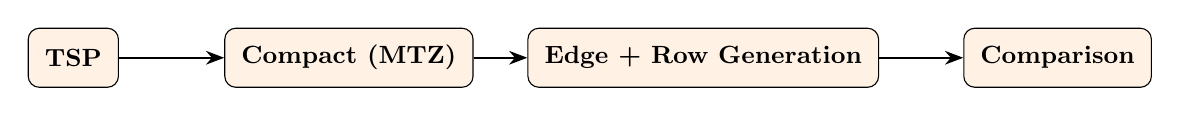
\begin{tikzpicture}[
  box/.style={draw, rounded corners, fill=orange!10,
              minimum height=0.75cm, font=\small\bfseries, inner xsep=6pt},
  arr/.style={-{Stealth}, thick}
]
  \node[box] (tsp) at (0, 0)   {TSP};
  \node[box] (weak) at (3.5, 0)  {Compact (MTZ)};
  \node[box] (row) at (8, 0)  {Edge + Row Generation};
  \node[box] (exp) at (12.5, 0) {Comparison};
  \draw[arr] (tsp) -- (weak);
  \draw[arr] (weak) -- (row);
  \draw[arr] (row) -- (exp);
\end{tikzpicture}
\end{center}

\medskip
\begin{itemize}
  \item \textbf{Motivation:} some formulations have exponentially many constraints
  \item \textbf{Row generation:} add \textbf{constraints} dynamically as they are violated
  \item \textbf{SCIP plugin:} the constraint handler
  \item \textbf{Application:} Traveling Salesman Problem (TSP)
\end{itemize}
\end{frame}

% ---------------------------------------------------------
% Frame 3: TSP Problem Statement
% ---------------------------------------------------------
\begin{frame}{Traveling Salesman Problem (TSP)}
\begin{columns}[T]
\begin{column}{0.52\textwidth}
\textbf{Given:} $n$ cities, pairwise distances $d_{ij}$

\textbf{Find:} shortest tour visiting each city exactly once, returning to start

\medskip
\begin{itemize}
  \item One of the most famous NP-hard problems
  \item Symmetric TSP: $d_{ij} = d_{ji}$ (undirected edges)
  \item We will compare two formulations:
    \begin{enumerate}
      \item Compact MTZ (polynomial constraints, weak LP)
      \item Extended DFJ (exponential constraints, strong LP)
    \end{enumerate}
\end{itemize}
\end{column}
\begin{column}{0.45\textwidth}
\centering
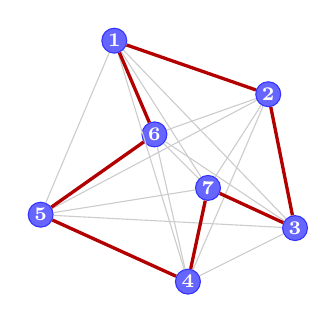
\begin{tikzpicture}[scale=0.85,
  city/.style={circle, draw=blue!80, fill=blue!60, inner sep=0pt,
               minimum size=9pt, font=\scriptsize\bfseries, text=white},
  tour/.style={very thick, red!70!black},
  nontour/.style={thin, gray!40}
]
  % City positions (7 cities, scattered with interior nodes)
  \node[city] (c1) at (-0.3, 2.3)  {1};
  \node[city] (c2) at (2.0, 1.5)   {2};
  \node[city] (c3) at (2.4,-0.5)   {3};
  \node[city] (c4) at (0.8,-1.3)   {4};
  \node[city] (c5) at (-1.4,-0.3)  {5};
  \node[city] (c6) at (0.3, 0.9)   {6};
  \node[city] (c7) at (1.1, 0.1)   {7};

  % All non-tour edges (complete graph background)
  \foreach \i in {1,...,7} {
    \foreach \j in {\i,...,7} {
      \ifnum\i<\j
        \draw[nontour] (c\i) -- (c\j);
      \fi
    }
  }

  % Optimal tour on top
  \draw[tour] (c1) -- (c6);
  \draw[tour] (c6) -- (c5);
  \draw[tour] (c5) -- (c4);
  \draw[tour] (c4) -- (c7);
  \draw[tour] (c7) -- (c3);
  \draw[tour] (c3) -- (c2);
  \draw[tour] (c2) -- (c1);
\end{tikzpicture}

\smallskip
{\scriptsize\color{red!70!black} Optimal tour in red;}
\end{column}
\end{columns}
\end{frame}

% ---------------------------------------------------------
% Frame 4: MTZ Formulation
% ---------------------------------------------------------
\begin{frame}{MTZ Formulation}
\begin{columns}[T]
\begin{column}{0.62\textwidth}
\textbf{Variables:} $x_{ij} \in \{0,1\}$ (directed edges), $u_i \in \mathbb{R}$ (positions)

\begin{align*}
  \min \quad & \sum_{i \neq j} d_{ij}\, x_{ij} \\
  \text{s.t.} \quad
    & \sum_{j \neq i} x_{ij} = 1 && \forall\, i \quad \text{(leave once)} \\
    & \sum_{i \neq j} x_{ij} = 1 && \forall\, j \quad \text{(enter once)} \\
    & u_i - u_j + n \cdot x_{ij} \le n - 1 && \forall\, i,j \neq 0 \quad \text{(MTZ)} \\
    & x_{ij} \in \{0,1\}
\end{align*}

\begin{itemize}
  \item $O(n^2)$ variables and constraints
  \item LP relaxation is \textbf{very weak}
\end{itemize}
\end{column}
\begin{column}{0.35\textwidth}
\centering
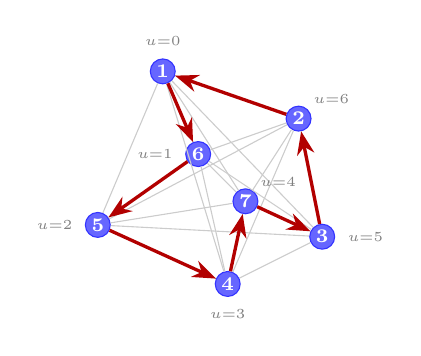
\begin{tikzpicture}[scale=0.75,
  city/.style={circle, draw=blue!80, fill=blue!60, inner sep=0pt,
               minimum size=9pt, font=\scriptsize\bfseries, text=white},
  tour/.style={very thick, red!70!black},
  nontour/.style={thin, gray!40}
]
  % 7 cities (same layout as Part 1)
  \node[city] (c1) at (-0.3, 2.3)  {1};
  \node[city] (c2) at (2.0, 1.5)   {2};
  \node[city] (c3) at (2.4,-0.5)   {3};
  \node[city] (c4) at (0.8,-1.3)   {4};
  \node[city] (c5) at (-1.4,-0.3)  {5};
  \node[city] (c6) at (0.3, 0.9)   {6};
  \node[city] (c7) at (1.1, 0.1)   {7};

  % Complete graph background
  \foreach \i in {1,...,7} {
    \foreach \j in {\i,...,7} {
      \ifnum\i<\j
        \draw[nontour] (c\i) -- (c\j);
      \fi
    }
  }

  % Directed tour
  \draw[tour, -{Stealth}] (c1) -- (c6);
  \draw[tour, -{Stealth}] (c6) -- (c5);
  \draw[tour, -{Stealth}] (c5) -- (c4);
  \draw[tour, -{Stealth}] (c4) -- (c7);
  \draw[tour, -{Stealth}] (c7) -- (c3);
  \draw[tour, -{Stealth}] (c3) -- (c2);
  \draw[tour, -{Stealth}] (c2) -- (c1);

  % MTZ position labels
  \node[font=\tiny, gray, above=1pt of c1] {$u{=}0$};
  \node[font=\tiny, gray, left=1pt of c6] {$u{=}1$};
  \node[font=\tiny, gray, left=1pt of c5]  {$u{=}2$};
  \node[font=\tiny, gray, below=1pt of c4] {$u{=}3$};
  \node[font=\tiny, gray, above right=-2pt of c7] {$u{=}4$};
  \node[font=\tiny, gray, right=1pt of c3] {$u{=}5$};
  \node[font=\tiny, gray, above right=-2pt of c2] {$u{=}6$};
\end{tikzpicture}

\smallskip
{\scriptsize $u_i$ values enforce a\\ single directed tour}
\end{column}
\end{columns}
\end{frame}

% ---------------------------------------------------------
% Frame 5: Exercise --- Compact MTZ
% ---------------------------------------------------------
\begin{frame}{Reference: Compact MTZ}
\begin{block}{Prerequisite}
Implement the MTZ formulation in Part 1 (Exercise 6) before starting Part 2.
\end{block}
\begin{itemize}
  \item File: \texttt{part1/ex06\_tsp\_mtz/tsp\_mtz.py}
  \item Test: \texttt{python part1/ex06\_tsp\_mtz/test\_tsp\_mtz.py}
\end{itemize}
\end{frame}

% ---------------------------------------------------------
% Frame 6: Edge Formulation with SECs
% ---------------------------------------------------------
\begin{frame}{Edge Formulation with SECs}
\begin{columns}[T]
\begin{column}{0.55\textwidth}
\textbf{Variables:} $x_e \in \{0,1\}$ for each undirected edge $e$

\begin{align*}
  \min \quad & \sum_{e \in E} d_e\, x_e \\
  \text{s.t.} \quad
    & \sum_{e \in \delta(v)} x_e = 2 && \forall\, v \in V
      \quad \text{(degree)} \\
    & \sum_{e \in E(S)} x_e \le |S| - 1 && \forall\, S \subset V \\
    & \quad 2 \le |S| \le n{-}1
      && \text{(SECs)} \\
    & x_e \in \{0,1\}
\end{align*}

\begin{itemize}
  \item \textbf{Exponentially many} SECs: $O(2^n)$ subsets
  \item \textbf{Much stronger} LP relaxation than MTZ
  \item Cannot add all upfront $\Rightarrow$ \textbf{row generation}
\end{itemize}
\end{column}
\begin{column}{0.42\textwidth}
\centering
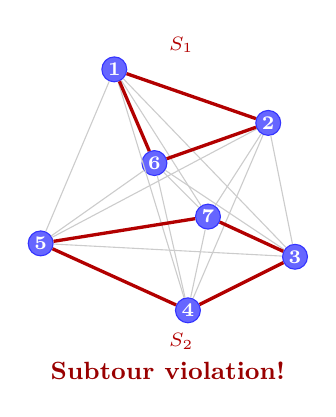
\begin{tikzpicture}[scale=0.85,
  city/.style={circle, draw=blue!80, fill=blue!60, inner sep=0pt,
               minimum size=9pt, font=\scriptsize\bfseries, text=white},
  subtour/.style={very thick, red!70!black},
  nontour/.style={thin, gray!40}
]
  % Same 7-city layout as the TSP intro slide
  \node[city] (c1) at (-0.3, 2.3)  {1};
  \node[city] (c2) at (2.0, 1.5)   {2};
  \node[city] (c3) at (2.4,-0.5)   {3};
  \node[city] (c4) at (0.8,-1.3)   {4};
  \node[city] (c5) at (-1.4,-0.3)  {5};
  \node[city] (c6) at (0.3, 0.9)   {6};
  \node[city] (c7) at (1.1, 0.1)   {7};

  % Faded complete graph
  \foreach \i in {1,...,7} {
    \foreach \j in {\i,...,7} {
      \ifnum\i<\j
        \draw[nontour] (c\i) -- (c\j);
      \fi
    }
  }

  % Subtour 1: {1, 2, 6}
  \draw[subtour] (c1) -- (c6) -- (c2) -- (c1);

  % Subtour 2: {3, 4, 5, 7}
  \draw[subtour] (c5) -- (c7) -- (c3) -- (c4) -- (c5);

  % Labels
  \node[font=\scriptsize\bfseries, red!70!black, above] at (0.7, 2.4)
    {$S_1$};
  \node[font=\scriptsize\bfseries, red!70!black, below] at (0.7, -1.5)
    {$S_2$};

  \node[font=\small\bfseries, red!60!black] at (0.5, -2.2)
    {Subtour violation!};
\end{tikzpicture}
\end{column}
\end{columns}
\end{frame}

% ---------------------------------------------------------
% Frame 7: Row Generation Paradigm
% ---------------------------------------------------------
\begin{frame}{Row Generation Paradigm}
\begin{center}
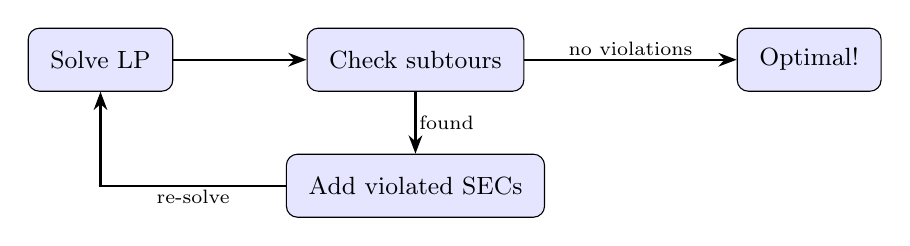
\begin{tikzpicture}[
  box/.style={draw, rounded corners, fill=blue!10,
              minimum height=0.8cm, font=\small, inner xsep=8pt},
  arr/.style={-{Stealth}, thick},
  lbl/.style={font=\scriptsize, fill=white, inner sep=1pt}
]
  \node[box] (solve) at (0, 0)      {Solve LP};
  \node[box] (check) at (4, 0)      {Check subtours};
  \node[box] (opt)   at (9, 0)      {Optimal!};
  \node[box] (add)   at (4, -1.6)   {Add violated SECs};

  \draw[arr] (solve) -- (check);
  \draw[arr] (check) -- node[lbl, above] {no violations} (opt);
  \draw[arr] (check) -- node[lbl, right] {found} (add);
  \draw[arr] (add.west) -| node[pos=0.25, lbl, below] {re-solve} (solve.south);
\end{tikzpicture}
\end{center}

\medskip
\begin{itemize}
  \item Start with a relaxed model (only degree constraints)
  \item Iteratively find and add violated constraints
  \item Converges to optimality without enumerating all $2^n$ SECs
\end{itemize}
\end{frame}

% ---------------------------------------------------------
% Frame 8: Constraint Handler Interface
% ---------------------------------------------------------
\begin{frame}[fragile]{Constraint Handler in SCIP}
SCIP implements row generation via the \textbf{constraint handler} plugin.

\medskip
\begin{table}
\centering\small
\begin{tabular}{lp{8cm}}
\toprule
\textbf{Callback} & \textbf{Purpose} \\
\midrule
\texttt{conscheck}  & Check if a candidate integer solution is feasible \\
\texttt{consenfolp} & Enforce constraints on LP solution; add cuts if violated \\
% \texttt{conslock}   & Declare variable locks (required; can be empty) \\
\bottomrule
\end{tabular}
\end{table}

\medskip
\begin{lstlisting}
class SubtourElimination(Conshdlr):
    def conscheck(self, constraints, solution, ...):
        # Find subtours; return FEASIBLE or INFEASIBLE
    def consenfolp(self, constraints, ...):
        # Add SEC for each subtour; return CONSADDED
\end{lstlisting}
\end{frame}

% ---------------------------------------------------------
% Frame 9: Exercise --- Subtour + Conshdlr
% ---------------------------------------------------------
\begin{frame}{Exercises: Subtour Detection \& Constraint Handler}
\begin{block}{Exercise 1 (optional): Subtour Detection}
Implement \texttt{find\_subtours()}: find connected components in the edge graph.
\end{block}
\begin{itemize}
  \item File: \texttt{part2/subtour.py}
  \item Test: \texttt{python part2/test\_subtour.py}
  \item Shortcut: use \texttt{networkx.connected\_components()} instead
\end{itemize}

\medskip
\begin{block}{Exercise 2: Constraint Handler}
Implement \texttt{conscheck} and \texttt{consenfolp} callbacks.
\end{block}
\begin{itemize}
  \item File: \texttt{part2/conshdlr\_subtour.py}
  \item Test: \texttt{python part2/test\_tsp.py}
\end{itemize}
\end{frame}

% ---------------------------------------------------------
% Frame 10: Exercise --- Experimental Comparison
% ---------------------------------------------------------
\begin{frame}{MTZ vs.\ Row Generation}
\begin{block}{Run the experiments}
\texttt{python experiments.py} compares both formulations on increasing sizes.
\end{block}

\medskip
\begin{columns}[T]
\begin{column}{0.48\textwidth}
\textbf{MTZ (compact)}
\begin{itemize}
  \item $O(n^2)$ constraints
  \item Very weak LP bound
  \item Many B\&B nodes needed
\end{itemize}
\end{column}
\begin{column}{0.48\textwidth}
\textbf{Row generation (SECs)}
\begin{itemize}
  \item Exponential constraints, added lazily
  \item LP bound often near-optimal
  \item Far fewer nodes
\end{itemize}
\end{column}
\end{columns}

\bigskip
\textbf{Key insight:} The LP relaxation bound is what matters. MTZ's LP
is significantly weaker, while the SEC LP bound is tight.
This gap widens as instance size grows.
\end{frame}

% ---------------------------------------------------------
% Frame 11: Summary
% ---------------------------------------------------------
\begin{frame}{Summary}
\textbf{What we covered:}
\begin{itemize}
  \item TSP: compact MTZ vs.\ edge formulation with SECs
  \item Row generation paradigm: add constraints on-the-fly
  \item SCIP constraint handler plugin (\texttt{conscheck}, \texttt{consenfolp})
  \item Exponential constraint families handled implicitly
\end{itemize}

\medskip
\textbf{Key takeaway:}
\begin{itemize}
  \item A strong LP relaxation can make a substantial difference in solving time
  \item Row generation lets us use formulations with exponentially many constraints
\end{itemize}

\medskip
\textbf{Part 3:} Branch-and-price for bin packing
\end{frame}

\end{document}
